\documentclass[12pt,a4paper]{article}
\usepackage[utf8]{inputenc}
\usepackage[russian]{babel}
\usepackage[OT1]{fontenc}
\usepackage{amsmath}
\usepackage{amsfonts}
\usepackage{amssymb}
\usepackage{graphicx}
\usepackage[left=2cm,right=2cm,top=2cm,bottom=2cm]{geometry}
\usepackage{calc}
\usepackage{wrapfig}
\usepackage{setspace}
\usepackage{indentfirst}
\usepackage{subfigure}


\title{
1.2.5.

Исследование вынужденной регулярной прецессии гироскопа
}

\author{Семёнов Андрей Б02-016}

\begin{document}

\date{17 марта 2021г.}
\maketitle

\newpage

	\textbf{Цель работы:} исследовать вынужденную прецессию гироскопа; установить зависимость скорости вынужденной прецессии гироскопа от величины момента сил, действующих на ось гироскопа; определить скорость вращения ротора гироскопа и сравнить ее со скоростью, рассчитанной по скорости прецессии.
	
	\textbf{В работе используются:} гироскоп в кардановом подвесе, секундомер, набор грузов, отдельный ротор гироскопа, цилиндр известной массы, крутильный маятник, штангенциркуль, линейка. 


\section{Теоретический материал}

Основные уравнения движения твердого тела можно записать в виде:

\begin{equation}
	\frac{d\vec{P}}{dt} = \vec{F}
	\label{eq:center_of_mass}
\end{equation}

\begin{equation}
	\frac{d\vec{L}}{dt} = \vec{M}
	\label{eq:moments_equation}
\end{equation}

Формула (\ref{eq:center_of_mass}) выражает закон движения центра масс, а формула (\ref{eq:moments_equation}) -- уравнение моментов, действующих на тело. Двух данных уравнений достаточно для описания состояния твердого тела.

Если сила $\vec{F}$ не зависит от угловой скорости вращения тела, а момент $\vec{M}$ от скорости поступательного движения тела, то уравнения (\ref{eq:center_of_mass}) и (\ref{eq:moments_equation}) можно рассматривать независимо друг от друга. В данной работе рассматривается только задача о вращении твердого тела.

Момент импульса твердого тела можно вычислить, используя формулу:
\begin{equation}
	\vec{L} = \vec{i}I_{x}\omega_{x} + \vec{j}I_{y}\omega_{y} + \vec{k}I_{z}\omega_{z},
\end{equation}
где $ I_{x},I_{y},I_{z} $ -- главные моменты инерции тела, $ \omega_{x}, \omega_{y}, \omega_{z} $ -- компоненты вектора угловой скорости  $\vec{\omega} $.

Быстро вращающееся тело, для которого:

	$$I_{z}\omega_{z} \gg I_{x}\omega_{x}, I_{y}\omega_{y}$$

принято называть \textit{гироскопом}. Гироскоп называется уравновешенным, если его центр масс неподвижен.

В силу (\ref{eq:moments_equation}), приращение момента импулься определяется интегралом:
\begin{equation}
	\Delta\vec{L} =  \int\vec{M}\\,dt
	\label{eq:integral_for_increment}
\end{equation}

Если момент внешних сил действует в течение короткого промежутка времени, из формулы (\ref{eq:integral_for_increment}) следует, что приращение $\vec{L}$ момента импулься значительно меньше самого момента импульса, т.е:

\begin{equation}
	\left| \Delta\vec{L} \right| \ll \left| \vec{L} \right|.
\end{equation}

Благодаря этому, гироскоп приобретает очень большую устойчивость, вызванную его быстрым вращением.

Если гироскоп уравновешен, то суммарный момент сил, действующих на него, равен 0. В таком случае, гироскоп не будет изменять своего положения в пространстве. Если на гироскоп в течение длительного времени будет действовать некоторый момент сил, отличный от нуля, то, согласно (\ref{eq:moments_equation}) гироскоп придет в движение. Мы не будем рассматривать действие моментов сил, которые вызовут ускорение или замедление гироскопа (т.е. моментов сил, которые не изменяют положения оси вращения гироскопа). Рассмотрим действия моментов сил, которые изменяют положение оси вращения гироскопа.

\begin{wrapfigure}[19]{r}{0.4\textwidth}
	\vspace{-2.5ex}
	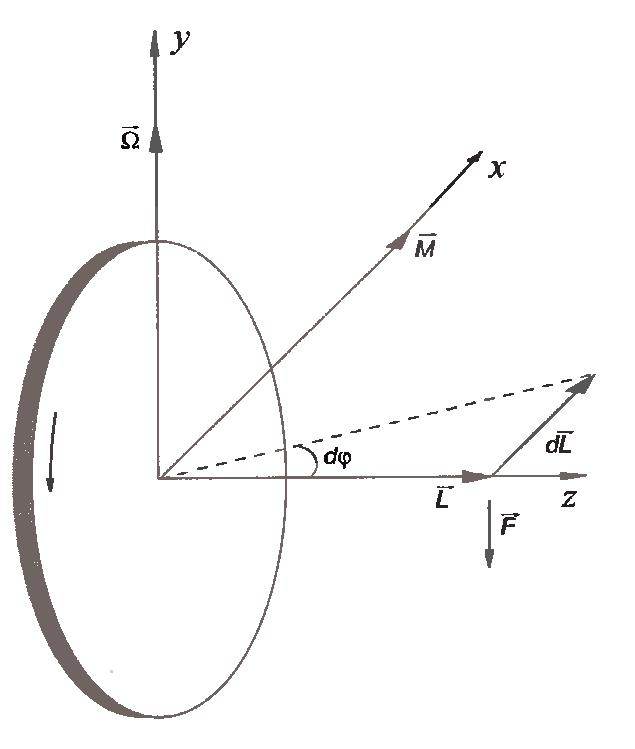
\includegraphics[width = 0.35\textwidth]{flywheel}
	\caption{Маховик.}
	\label{fig:flywheel}
\end{wrapfigure}

Рассмотрим маховик, вращающийся вокруг оси z. (Рис. \ref{fig:flywheel}). Будем считать, что 
$$ \omega_{z} = \omega_{0},\qquad \omega_{x} = \omega_{y} = 0.$$

Пусть ось вращения повернулась в плоскости \textit{zx} по направлению в оси \textit{x} на бесконечно малый угол $d\varphi$. Такой поворот означает добавочное вращение маховика вокруг оси \textit{y}, так что 
$$ d\varphi = \Omega\,dt, $$
где $ \Omega $ -- угловая скорость такого вращения. Будем предполагать, что
\begin{equation}
	L_{\Omega} \ll L_{\omega_{0}}
	\label{eq:condition_for_rotate}
\end{equation}

Это означает, что момент импульса маховика, равный $I_{z}\omega_{0}$ до приложения внешних сил, только повернется в плоскости \textit{zx} по направлению к оси \textit{x} не изменяя своей величины. Таким образом,

\begin{equation}
	\left|d\vec{L}\right| = Ld\varphi = I\Omega\,dt
	\label{eq:increment_moment_of_impulse}
\end{equation}


Записывая выражение (\ref{eq:increment_moment_of_impulse}) в виде векторного произведения, получаем:

\begin{equation}
	\frac{d\vec{L}}{dt} = \vec{\Omega} \times \vec{L}
\end{equation}

Окончательно, используя (\ref{eq:moments_equation}), получаем:

\begin{equation}
	\vec{M} = \vec{\Omega} \times \vec{L}
	\label{eq:rotation_by_moments_of_force}
\end{equation}

Формула (\ref{eq:rotation_by_moments_of_force}) справедлива, если выполнено условие (\ref{eq:condition_for_rotate}).
Данная формула позволяет определить, момент сил $ \vec{M}, $ который нужно приложить к маховику, чтобы вызвать вращение маховика с угловой скоростью $\vec{\Omega}$.

Под действием момента внешних сил $\vec{M}$ ось гироскопа медленно вращается вокруг оси \textit{y} с угловой скоростью $\vec{\Omega}$. Такое движение называют \textit{прецессией гироскопа}.

Для изучения регулярной прецессии уравновешенного гироскопа к его оси подвешивают дополнительные грузы. Это смещает общий центр масс и создает момент сил тяжести, вызывающий прецессию. Скорость прецессии в этом случае может быть найдена по формуле:

\begin{equation}
	\Omega = \frac{mgl}{I_{z}\omega_{0}},
	\label{eq:teor_equation_omega}
\end{equation} 
где m -- масса груза, l -- расстояние от центра карданова подвеса до точки крепления груза на оси гироскопа. (Рис. \ref{fig:facility})

Для выполнения работы используется гироскоп (Рис. \ref{fig:facility}), закрепленный в карданном подвесе (Рис. \ref{fig:Cardan_suspension}).


\begin{figure}[ht!]  
	\vspace{-4ex} 
	\centering 
	\subfigure[]{
		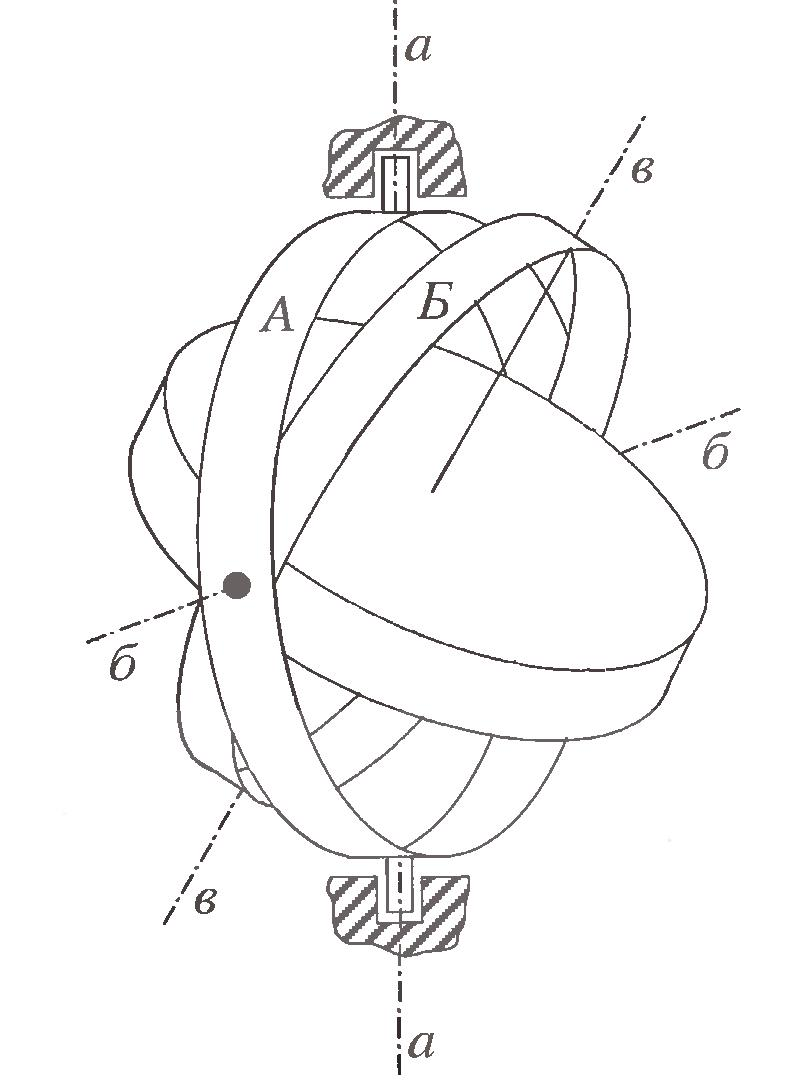
\includegraphics[width=0.29\linewidth]{Cardan_suspension} 	
			\label{fig:Cardan_suspension}}  
	\hspace{4ex}
	\subfigure[]{
		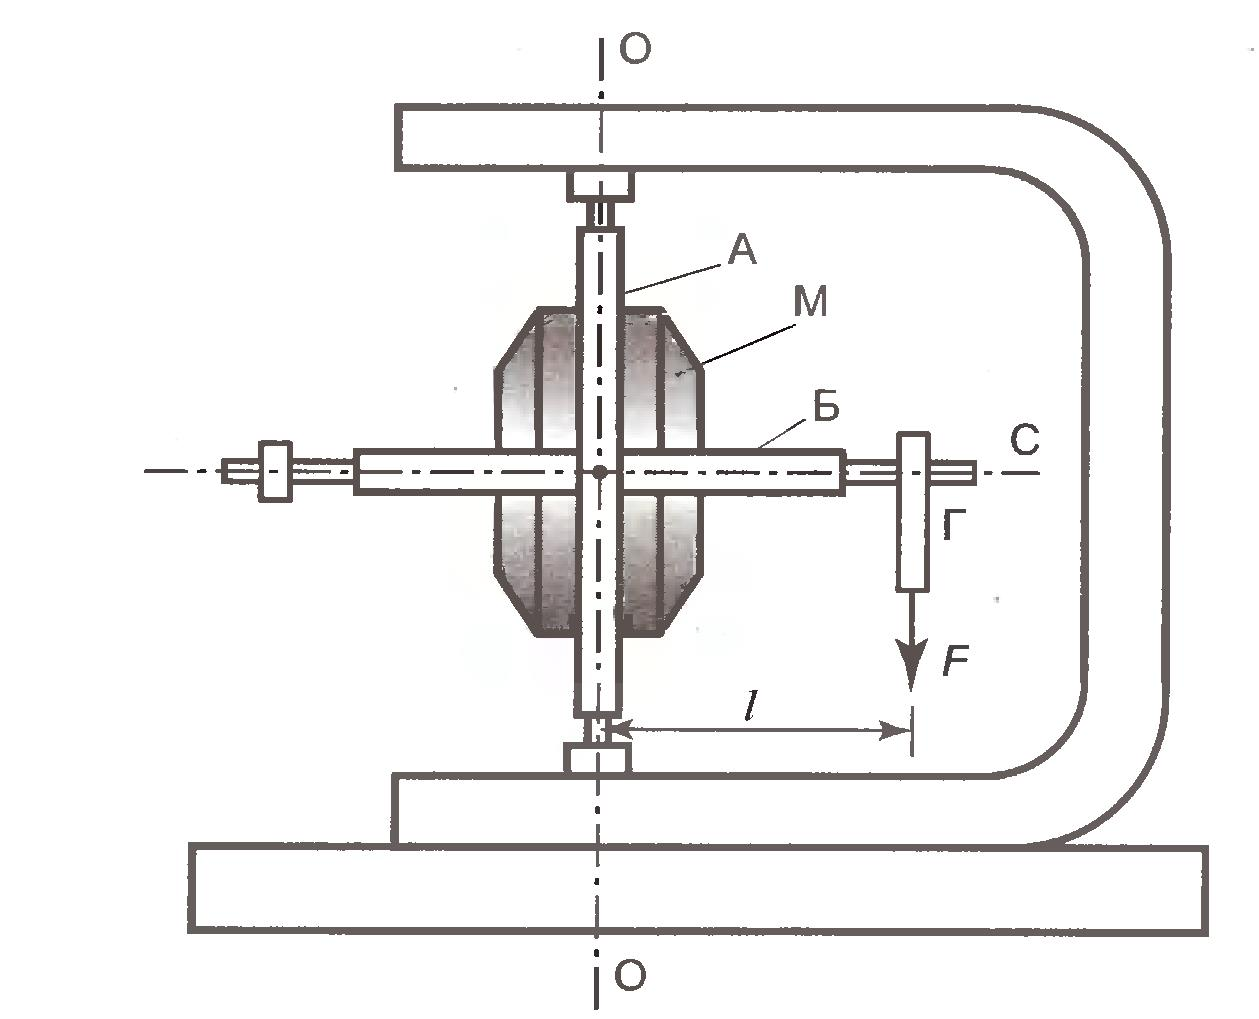
\includegraphics[width=0.45\linewidth]{facility} 
			\label{fig:facility} }  
	\caption{а) Гироскоп, закрепленный в карданном подвесе. б) Схема устройства гироскопа.}
\end{figure}

Ротором гироскопа (Рис. \ref{fig:facility}) является ротор электромотора М. Кожух мотора скреплен с кольцом Б (Рис. \ref{fig:Cardan_suspension}). Мотор с кольцом Б может вращаться в кольце А вокруг горизонтальной оси бб, которое может вращаться относительно оси аа. Рычаг С направлен по оси симметрии ротора. на рычаг подвешивают грузы Г.


\section{Выполнение работы}

\end{document}